\documentclass[12pt]{article}

%%%%%%%%%%%%%%%%%%%%%%%%%%%%%%%%%%%%%%%%%
% Lachaise Assignment
% Structure Specification File
% Version 1.0 (26/6/2018)
%
% This template originates from:
% http://www.LaTeXTemplates.com
%
% Authors:
% Marion Lachaise & François Févotte
% Vel (vel@LaTeXTemplates.com)
%
% License:
% CC BY-NC-SA 3.0 (http://creativecommons.org/licenses/by-nc-sa/3.0/)
% 
%%%%%%%%%%%%%%%%%%%%%%%%%%%%%%%%%%%%%%%%%

%----------------------------------------------------------------------------------------
%	PACKAGES AND OTHER DOCUMENT CONFIGURATIONS
%----------------------------------------------------------------------------------------

\usepackage{amsmath,amsfonts,stmaryrd,amssymb} % Math packages

\usepackage{enumerate} % Custom item numbers for enumerations

\usepackage[ruled]{algorithm2e} % Algorithms

\usepackage[framemethod=tikz]{mdframed} % Allows defining custom boxed/framed environments

\usepackage{listings} % File listings, with syntax highlighting
\lstset{
	basicstyle=\ttfamily, % Typeset listings in monospace font
}

%----------------------------------------------------------------------------------------
%	DOCUMENT MARGINS
%----------------------------------------------------------------------------------------

\usepackage{geometry} % Required for adjusting page dimensions and margins

\geometry{
	paper=a4paper, % Paper size, change to letterpaper for US letter size
	top=2.5cm, % Top margin
	bottom=3cm, % Bottom margin
	left=2.5cm, % Left margin
	right=2.5cm, % Right margin
	headheight=14pt, % Header height
	footskip=1.5cm, % Space from the bottom margin to the baseline of the footer
	headsep=1.2cm, % Space from the top margin to the baseline of the header
	%showframe, % Uncomment to show how the type block is set on the page
}

%----------------------------------------------------------------------------------------
%	FONTS
%----------------------------------------------------------------------------------------

\usepackage[utf8]{inputenc} % Required for inputting international characters
\usepackage[T1]{fontenc} % Output font encoding for international characters

\usepackage{XCharter} % Use the XCharter fonts

%----------------------------------------------------------------------------------------
%	COMMAND LINE ENVIRONMENT
%----------------------------------------------------------------------------------------

% Usage:
% \begin{commandline}
%	\begin{verbatim}
%		$ ls
%		
%		Applications	Desktop	...
%	\end{verbatim}
% \end{commandline}

\mdfdefinestyle{commandline}{
	leftmargin=10pt,
	rightmargin=10pt,
	innerleftmargin=15pt,
	middlelinecolor=black!50!white,
	middlelinewidth=2pt,
	frametitlerule=false,
	backgroundcolor=black!5!white,
	frametitle={Command Line},
	frametitlefont={\normalfont\sffamily\color{white}\hspace{-1em}},
	frametitlebackgroundcolor=black!50!white,
	nobreak,
}

% Define a custom environment for command-line snapshots
\newenvironment{commandline}{
	\medskip
	\begin{mdframed}[style=commandline]
}{
	\end{mdframed}
	\medskip
}

%----------------------------------------------------------------------------------------
%	FILE CONTENTS ENVIRONMENT
%----------------------------------------------------------------------------------------

% Usage:
% \begin{file}[optional filename, defaults to "File"]
%	File contents, for example, with a listings environment
% \end{file}

\mdfdefinestyle{file}{
	innertopmargin=1.6\baselineskip,
	innerbottommargin=0.8\baselineskip,
	topline=false, bottomline=false,
	leftline=false, rightline=false,
	leftmargin=2cm,
	rightmargin=2cm,
	singleextra={%
		\draw[fill=black!10!white](P)++(0,-1.2em)rectangle(P-|O);
		\node[anchor=north west]
		at(P-|O){\ttfamily\mdfilename};
		%
		\def\l{3em}
		\draw(O-|P)++(-\l,0)--++(\l,\l)--(P)--(P-|O)--(O)--cycle;
		\draw(O-|P)++(-\l,0)--++(0,\l)--++(\l,0);
	},
	nobreak,
}

% Define a custom environment for file contents
\newenvironment{file}[1][File]{ % Set the default filename to "File"
	\medskip
	\newcommand{\mdfilename}{#1}
	\begin{mdframed}[style=file]
}{
	\end{mdframed}
	\medskip
}

%----------------------------------------------------------------------------------------
%	NUMBERED QUESTIONS ENVIRONMENT
%----------------------------------------------------------------------------------------

% Usage:
% \begin{question}[optional title]
%	Question contents
% \end{question}

\mdfdefinestyle{question}{
	innertopmargin=1.2\baselineskip,
	innerbottommargin=0.8\baselineskip,
	roundcorner=5pt,
	nobreak,
	singleextra={%
		\draw(P-|O)node[xshift=1em,anchor=west,fill=white,draw,rounded corners=5pt]{%
		Question \theQuestion\questionTitle};
	},
}

\newcounter{Question} % Stores the current question number that gets iterated with each new question

% Define a custom environment for numbered questions
\newenvironment{question}[1][\unskip]{
	\bigskip
	\stepcounter{Question}
	\newcommand{\questionTitle}{~#1}
	\begin{mdframed}[style=question]
}{
	\end{mdframed}
	\medskip
}

%----------------------------------------------------------------------------------------
%	WARNING TEXT ENVIRONMENT
%----------------------------------------------------------------------------------------

% Usage:
% \begin{warn}[optional title, defaults to "Warning:"]
%	Contents
% \end{warn}

\mdfdefinestyle{warning}{
	topline=false, bottomline=false,
	leftline=false, rightline=false,
	nobreak,
	singleextra={%
		\draw(P-|O)++(-0.5em,0)node(tmp1){};
		\draw(P-|O)++(0.5em,0)node(tmp2){};
		\fill[black,rotate around={45:(P-|O)}](tmp1)rectangle(tmp2);
		\node at(P-|O){\color{white}\scriptsize\bf !};
		\draw[very thick](P-|O)++(0,-1em)--(O);%--(O-|P);
	}
}

% Define a custom environment for warning text
\newenvironment{warn}[1][Warning:]{ % Set the default warning to "Warning:"
	\medskip
	\begin{mdframed}[style=warning]
		\noindent{\textbf{#1}}
}{
	\end{mdframed}
}

%----------------------------------------------------------------------------------------
%	INFORMATION ENVIRONMENT
%----------------------------------------------------------------------------------------

% Usage:
% \begin{info}[optional title, defaults to "Info:"]
% 	contents
% 	\end{info}

\mdfdefinestyle{info}{%
	topline=false, bottomline=false,
	leftline=false, rightline=false,
	nobreak,
	singleextra={%
		\fill[black](P-|O)circle[radius=0.4em];
		\node at(P-|O){\color{white}\scriptsize\bf i};
		\draw[very thick](P-|O)++(0,-0.8em)--(O);%--(O-|P);
	}
}

% Define a custom environment for information
\newenvironment{info}[1][Info:]{ % Set the default title to "Info:"
	\medskip
	\begin{mdframed}[style=info]
		\noindent{\textbf{#1}}
}{
	\end{mdframed}
}

\title{VE527: Assignment \#2} % Title of the assignment
\author{Name: Chang Meng\\Student ID:\@\texttt{118370910019}}
\date{\today}

\begin{document}

    \maketitle

    \section{(12\%) Quadratic Wirelength Calculation}

        Consider the following simple placement of 5 gates in a small 6$\times$6 grid.

        \begin{center}
            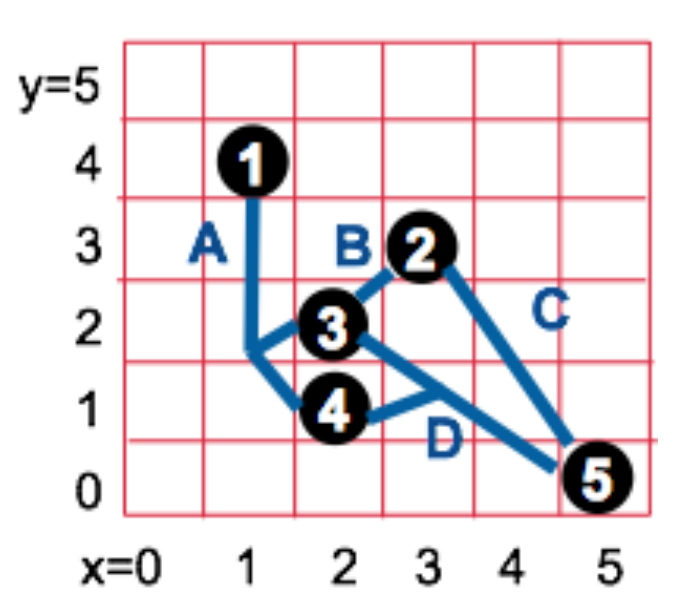
\includegraphics[width = 1.80in, height = 1.60in]{figure1.png}
        \end{center}

        \noindent
        Each gate is drawn as a circle with number (1\-5). Assumer the gate is located at the
        center of the grid cell, and its (X, Y) coordinates are taken from the column (X) and
        row (Y) coordinates in the figure. There are 4 nets, labeled A, B, C and D, connected
        as follows:

        \begin{itemize}
            \item Net A:\@ gates 1, 3, 4
            \item Net B:\@ gates 2, 3
            \item Net C:\@ gates 2, 5
            \item Net D:\@ gates 3, 4, 5
        \end{itemize}

        \noindent
        For this placement, what is its total quadratic Wirelength?

        \noindent
        \\Answer:\\

        \noindent
        For Net A, it has 3 points, so the weight = 1/2, and its quadratic wirelength is:
        \[\frac{1}{2}[{(1-2)}^2+{(4-2)}^2]+\frac{1}{2}[{(1-2)}^2+{(4-1)}^2]+
        \frac{1}{2}[{(2-2)}^2+{(2-1)}^2]=8\]
        For Net B, it has 2 points, so the weight = 1, and its quadratic wirelength is:
        \[[{(3-2)}^2+{(3-2)}^2]=2\]
        For Net C, it has 2 points, so the weight = 1, and its quadratic wirelength is:
        \[[{(3-5)}^2+{(3-0)}^2]=13\]
        For Net D, it has 3 points, so the weight = 2, and its quadratic wirelength is:
        \[\frac{1}{2}[{(2-2)}^2+{(2-1)}^2]+\frac{1}{2}[{(2-5)}^2+{(2-0)}^2]+
        \frac{1}{2}[{(2-5)}^2+{(1-0)}^2]=12\]
        The total quadratic wirelength is
        \[8+2+13+12=35\]

    \section{(24\%) Quadratic Placement}

        Consider the following simple netlist of 4 gates and 3 pads, to be placed in a square
        that extends from X = 0 to 1, and Y = 0 to 1. Assume that these are the final 2-point
        nets to be used in a quadratic placement. All nets have weight 1.0, except the two
        nets from gates 3 to 4 and the net from gate 4 to the pad at (0.25, 1). Their weights
        are 10 and 20, respectively. To perform a quadratic placement, we solve two systems
        of linear equations $AX=b_X$ and $AY=b_Y$.

        \begin{center}
            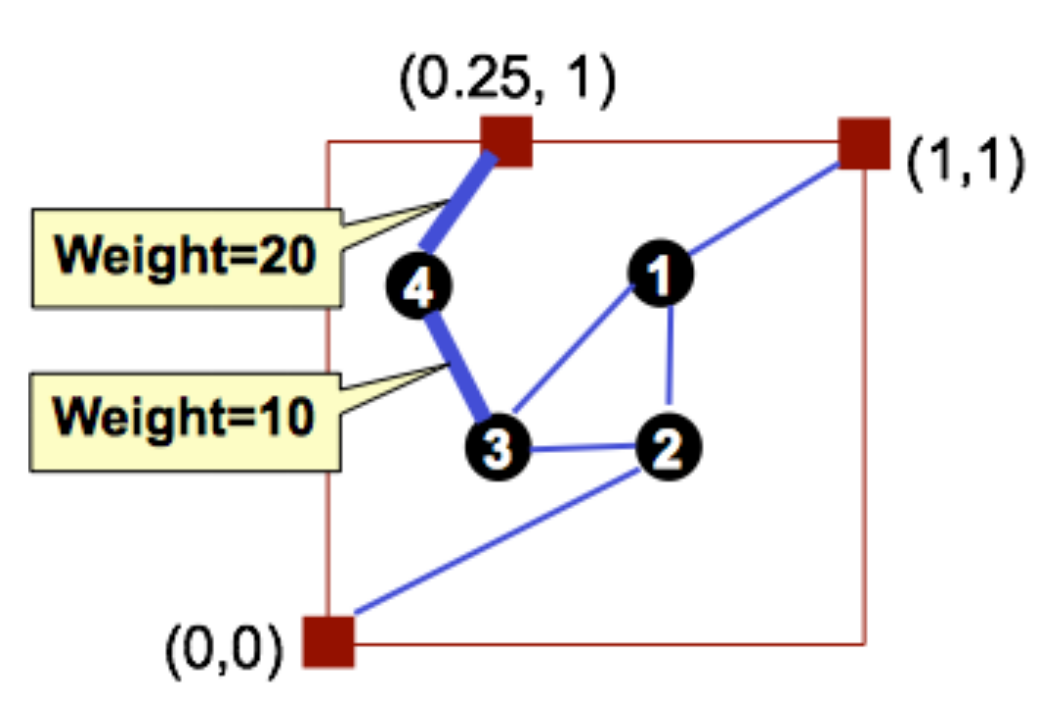
\includegraphics[width = 2.60in, height = 1.60in]{figure2.png}
        \end{center}

        \begin{enumerate}[(a)]
            \item (8\%) Build the matrix $A$ using the recipe from the lecture.
            \item (8\%) Build the vectors $b_X$ and $b_Y$ using the recipe from the lecture.
            \item (4\%) Solve for the $(X, Y)$ coordinates for gates 1, 2, 3, and 4. You can
                solve this any way you like (i.e., you can use your favorite solver).
            \item (4\%) After the initial placement, now suppose we want to do recursive
                partitioning and we divide the chip in half \textbf{\underline{vertically}}.
                We want to next formulate a new, smaller QP problem in the region left to the
                cutline. Which gates should be assigned to this left region? Which gates/pads
                should be propagated to the vertical cutline as pseudo-pads?
        \end{enumerate}

        \noindent
        Answer:

        \begin{enumerate}[(a)]
            \item The connectivity matrix is:
                \[C=
                    \left[
                        \begin{array}{cccc}
                            0 & 1 & 1 & 0\\
                            1 & 0 & 1 & 0\\
                            1 & 1 & 0 & 10\\
                            0 & 0 & 10 & 0
                        \end{array}
                    \right]
                \]
                Then we can get:
                \[A=
                    \left[
                        \begin{array}{cccc}
                            3 & -1 & -1 & 0\\
                            -1 & 3 & -1 & 0\\
                            -1 & -1 & 12 & -10\\
                            0 & 0 & -10 & 30
                        \end{array}
                    \right]
                \]
            \item
                Gate 1 connects to pad (1, 1) with weight 1,
                \[b_X[1]=1\times1=1, b_Y[1]=1\times1=1\]
                Gate 2 connects to pad (0, 0) with weight 1,
                \[b_X[2]=1\times0=0, b_Y[2]=1\times0=0\]
                Gate 4 connects to pad (0.25, 1) with weight 20,
                \[b_X[4]=20\times0.25=5, b_Y[4]=20\times1=20\]
                So, we can get:
                \[b_X=
                    \left[
                        \begin{array}{c}
                            1\\0\\0\\5
                        \end{array}
                    \right],
                b_Y=
                    \left[
                        \begin{array}{c}
                            1\\0\\0\\20
                        \end{array}
                    \right]
                \]
            \item
                The solution of the equations are:
                \[X=
                    \left[
                        \begin{array}{cccc}
                            \frac{95}{184} & \frac{49}{184} & \frac{13}{46} & \frac{6}{23}
                        \end{array}
                    \right],
                Y=
                    \left[
                        \begin{array}{cccc}
                            \frac{155}{184} & \frac{109}{184} & \frac{43}{46} & \frac{45}{46}
                        \end{array}
                    \right]
                \]
                So the coordinates are: $(X_1, Y_1)=(0.52, 0.84)$, $(X_2, Y_2)=(0.27, 0.59)$,
                $(X_3, Y_3)=(0.28, 0.93)$, $(X_4, Y_4)=(0.26, 0.98)$
            \item
                We sorted the gates by their X coordinates and get a sequence of $X_4$, $X_2$,
                $X_3$, $X_1$. So gate 2 and gate 4 will be assigned to the left region. Gate 1
                and gate 3 will be propagated to the vertical cutline as pseudo-pads because
                they are both connected to gate 2 in the left region.
        \end{enumerate}

    \section{(6\%) Maze Routing: Basics}

        Which of the following statements about maze routing are correct?

        \begin{enumerate}[a)]
            \item Maze routing can only handle a maximum of two routing layers.
            \item Maze routing routes a set of nets simultaneously.
            \item To efficiently find a minimum-cost item from the wavefront, we can use a
                data structure such as a min heap.
            \item If we add to the cost function a predictor that is a lower bound on the
                actual extra pathcost to the target, then maze routing will still find the
                minimum cost path. This kind of search is called A* search.
        \end{enumerate}

        \noindent
        Answer:\\

        c), d) are correct.

    \section{(12\%) Basic 2-point net routing in 1 layer}

        Consider the simple 6$\times$6 routing grid shown below. We label a source S cell, a
        target T cell, and several obstacle cells in black. All white cells have unit cost.
        Use the simple unit-cost maze routing expansion method, and perform wavefront
        expansion by hand on the grid, to find a route from S to T. Mark the route you obtain.
        What is the pathcost of this route?

        \begin{center}
            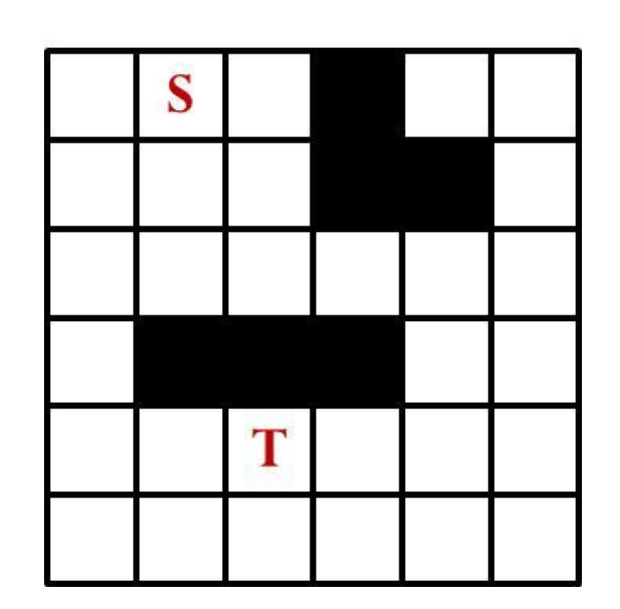
\includegraphics[width = 1.80in, height = 1.60in]{figure3.png}
        \end{center}

        \noindent
        Answer:\\

        \noindent
        The expansion process is like this:

        \begin{center}
            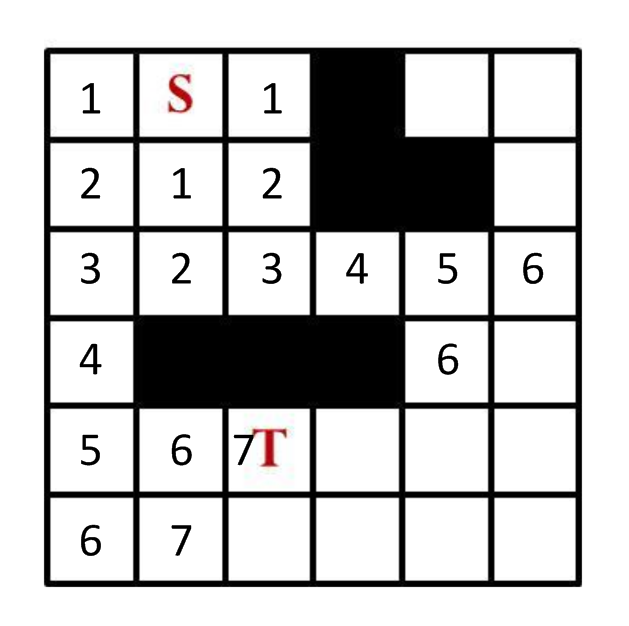
\includegraphics[width = 1.80in, height = 1.60in]{figure4.png}
        \end{center}

        \noindent
        The route is shown in the graph:

        \begin{center}
            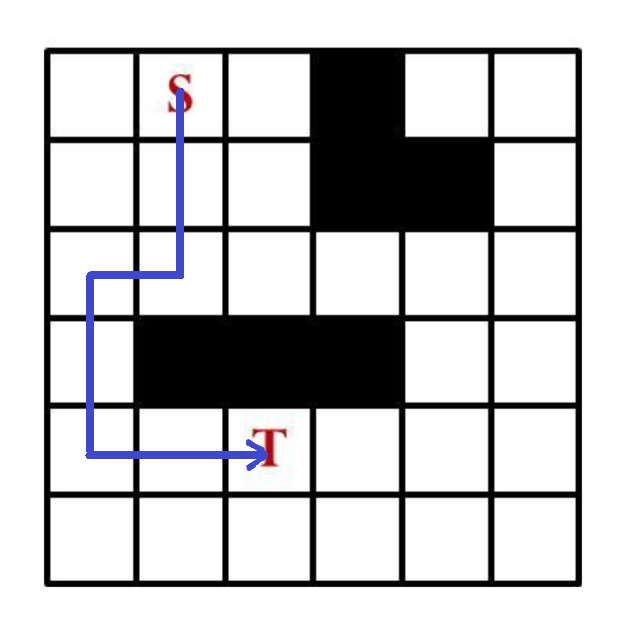
\includegraphics[width = 1.80in, height = 1.60in]{figure5.png}
        \end{center}

        \noindent
        The pathcost of this route is 7.

    \section{(20\%) Multi-point net routing in 1 layer}

        Consider the simple 6$\times$6 grid shown below. We label one source cell S, two
        target cells T, and several obstacle cells in black. All white cells have unit cost.
        Use the simple unit-cost maze routing expansion method and the techinique for
        completing mutil-point nets, and perform wavefront expansion by hand on the grid,
        to find a route for this 3-point net. Mark the route you obtain. What is the total
        pathcost of this route?

        \begin{center}
            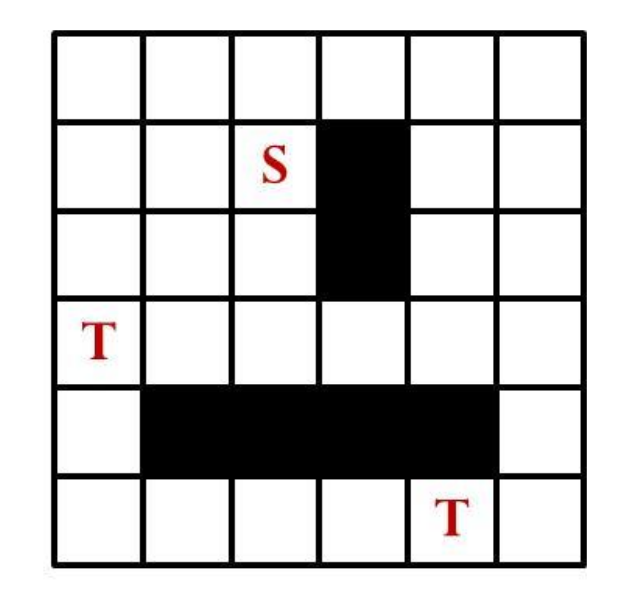
\includegraphics[width = 1.80in, height = 1.60in]{figure6.png}
        \end{center}

        \noindent
        Answer:\\

        \noindent
        We expand from S and find the T in the left first, as is shown in the following
        figure:

        \begin{center}
            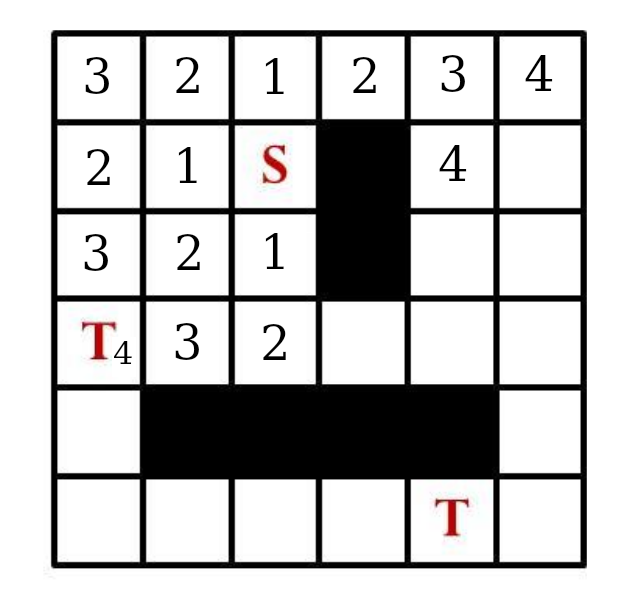
\includegraphics[width = 1.80in, height = 1.60in]{figure7.png}
        \end{center}

        \noindent
        Then we choose one of the shortest paths from S to T in the left like this:

        \begin{center}
            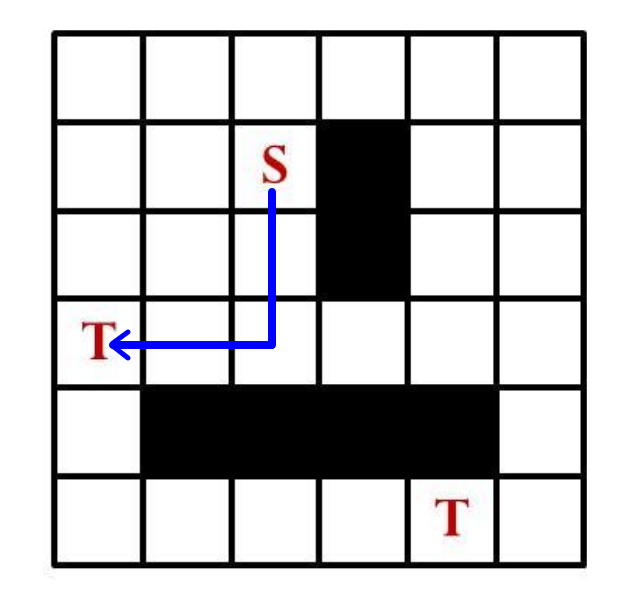
\includegraphics[width = 1.80in, height = 1.60in]{figure8.png}
        \end{center}

        \noindent
        We set the cost on the path above as 0, and expand from the path again:

        \begin{center}
            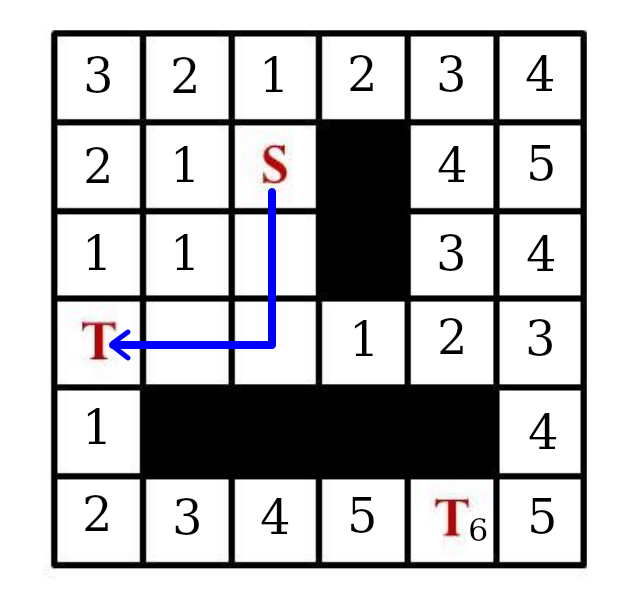
\includegraphics[width = 1.80in, height = 1.60in]{figure9.png}
        \end{center}

        \noindent
        Finally, we obtain a route with total pathcost = 10

        \begin{center}
            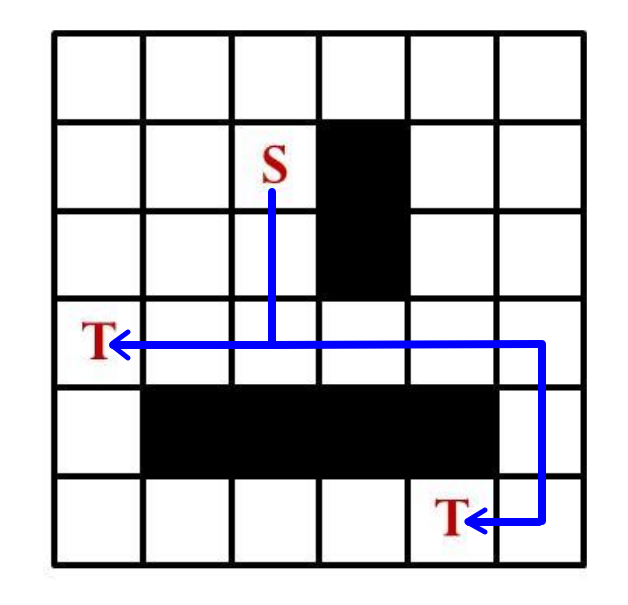
\includegraphics[width = 1.80in, height = 1.60in]{figure10.png}
        \end{center}

    \section{(10\%) Routing with non-unit costs in 1 layer}

        Consider the simple 6$\times$6 routing grid shown below. We label one source S, one
        target T, and several non-unit-cost cells in pink with \textbf{\underline{integer}}
        cost K. All white cells have unit cost. Assume your router uses the
        Cheapest-cell-first maze routing expansion algorithm. Suppose that your router finally
        returns a path that \textbf{avoids} all non-unit-cost cells. In this case, K must be
        large enough so that the path through the unit-cost cells will be cheaper than the path
        through the unit-cost cells will be cheaper than the path through the non-unit-cost
        cells. Then, what is minimum value of K?

        \begin{center}
            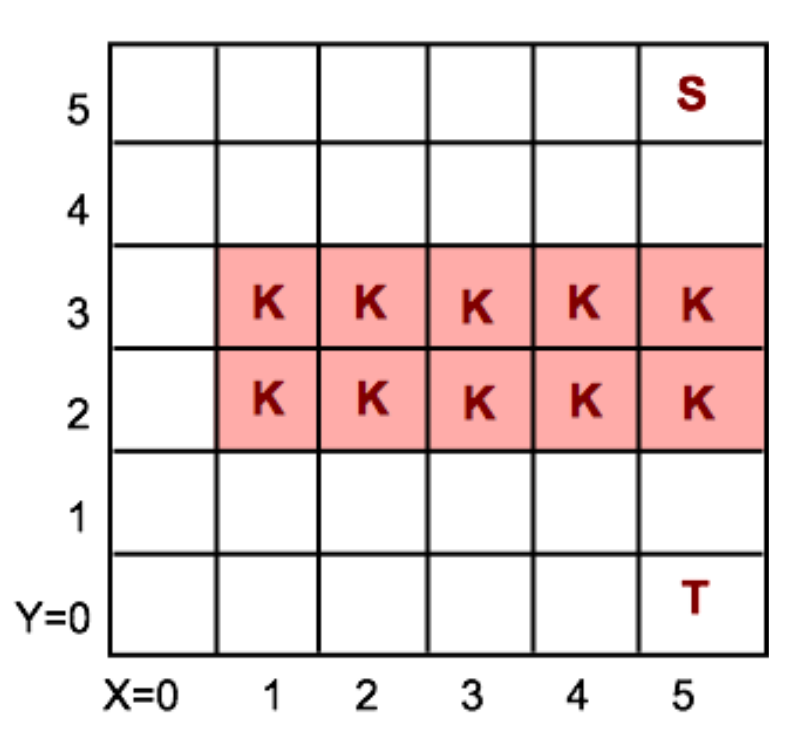
\includegraphics[width = 1.90in, height = 1.70in]{figure11.png}
        \end{center}

        \noindent
        Answer:\\

        \noindent
        If we treat non-unit-cost grids as obstacle, it will expand as is shown below, we can
        get a path avoiding all non-unit-cost cells with a cost of 15.

        \begin{center}
            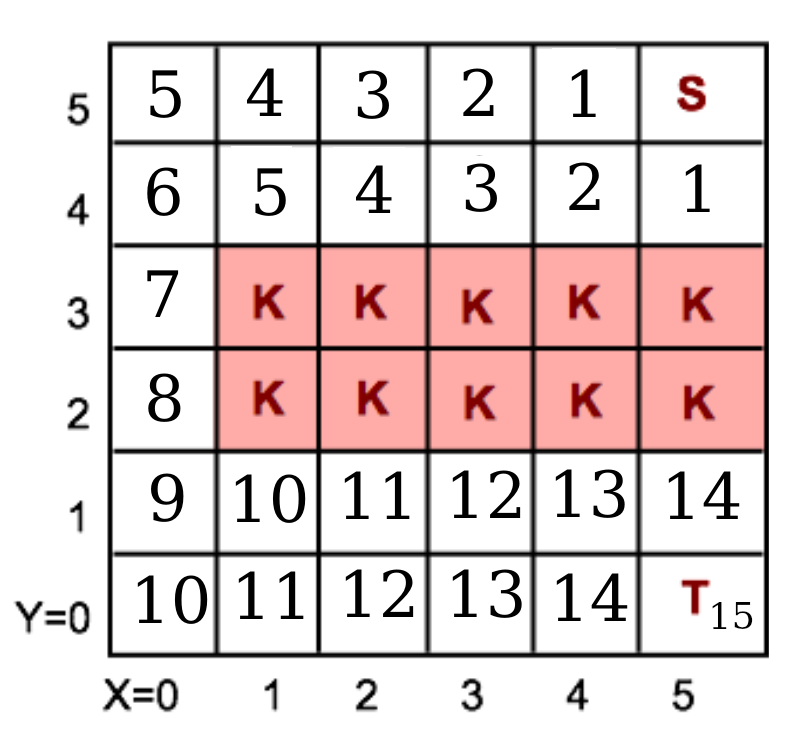
\includegraphics[width = 1.90in, height = 1.70in]{figure12.png}
        \end{center}

        \noindent
        The shortest path with non-unit-cost is like the following figure, and its cost is
        $2K+3$.

        \begin{center}
            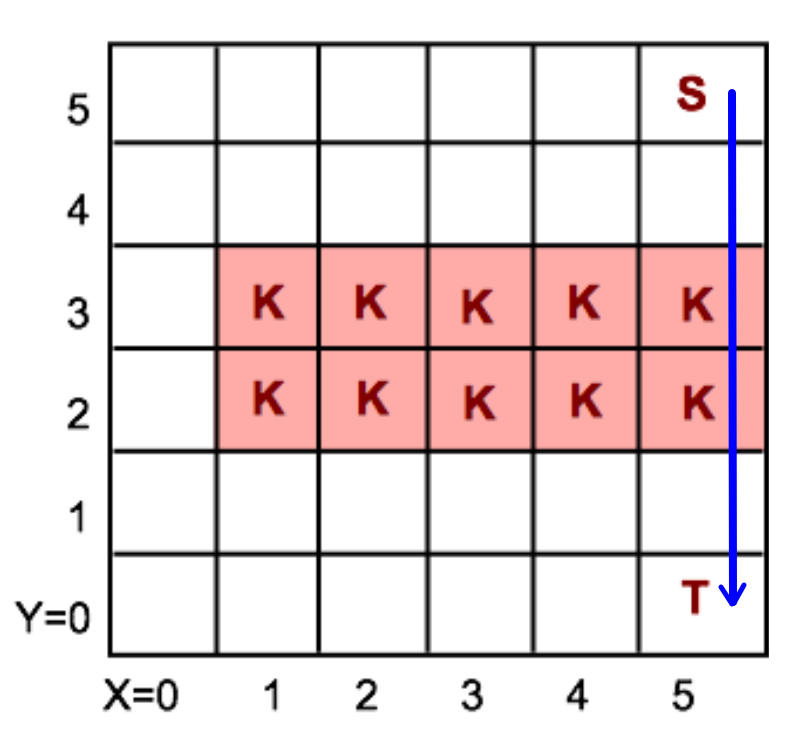
\includegraphics[width = 1.90in, height = 1.70in]{figure13.png}
        \end{center}

        To avoid non-unit-cost cells,
        \[2K+3>15, K>6\]

        So the minimum value of K is 7.


    \section{(16\%) Cheapest-cell-first expansion}

        Consider the simple 6$\times$6 routing grid shown below. We label one source S and one
        target T. The white cells have cost 1, the green cells have cost 2, and the pink cells
        have cost 3. Apply the Cheapest-cell-first maze routing expansion algorithm to find a
        route from S to T. Mark the route you have found. What is its pathcost?

        \begin{center}
            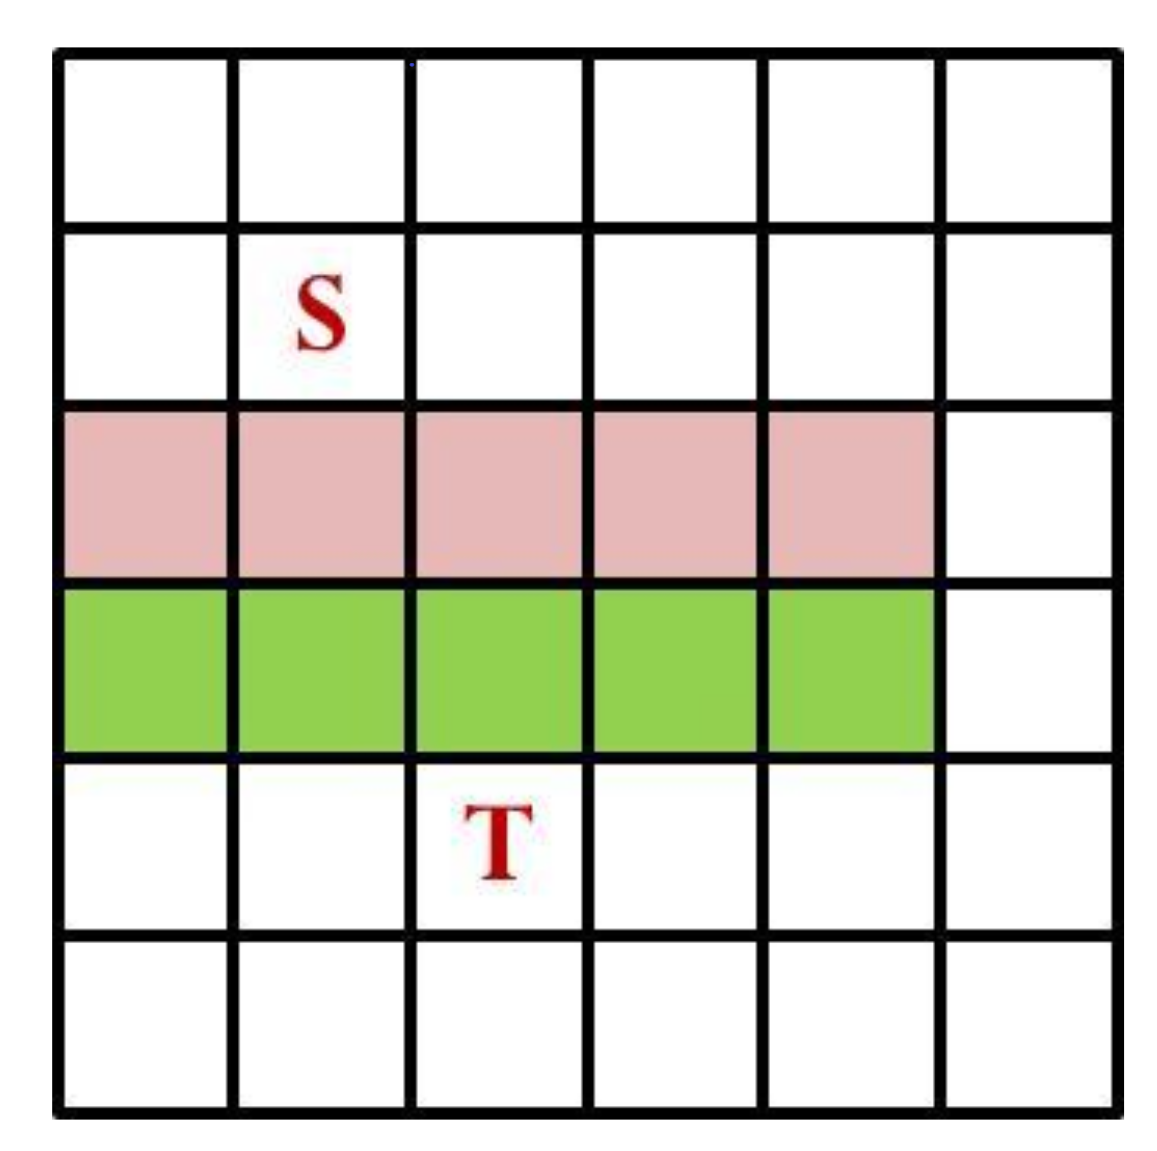
\includegraphics[width = 1.90in, height = 1.70in]{figure14.png}
        \end{center}

        \noindent
        Answer:\\

        The expansion process and the founded route is shown below:

        \begin{center}
            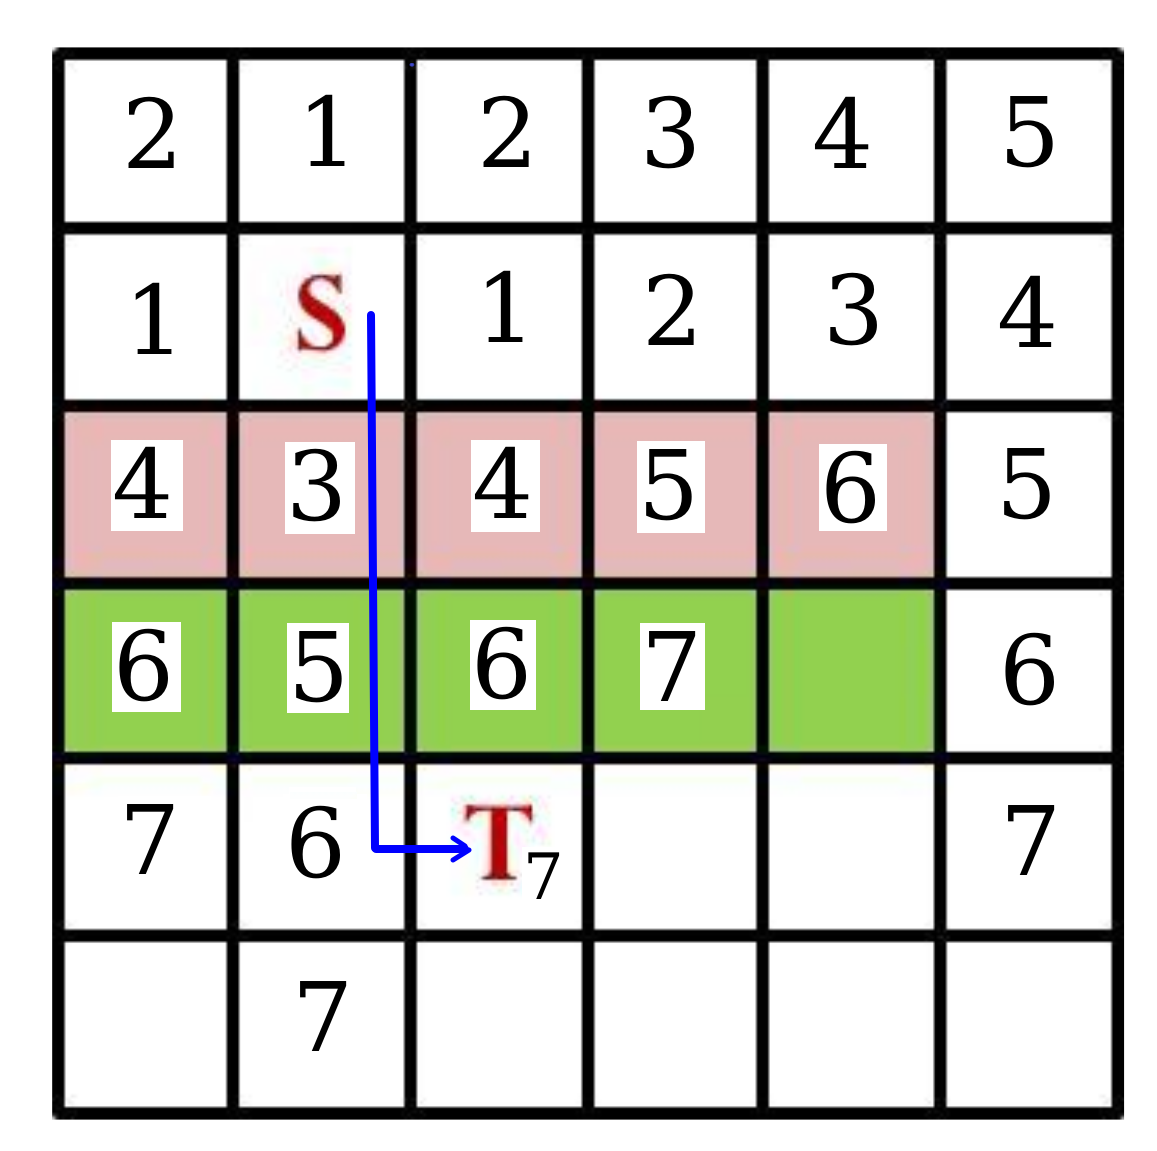
\includegraphics[width = 1.90in, height = 1.70in]{figure15.png}
        \end{center}

        Notably, to reconstruct the final path, I record the parents for each grids like this
        graph:

        \begin{center}
            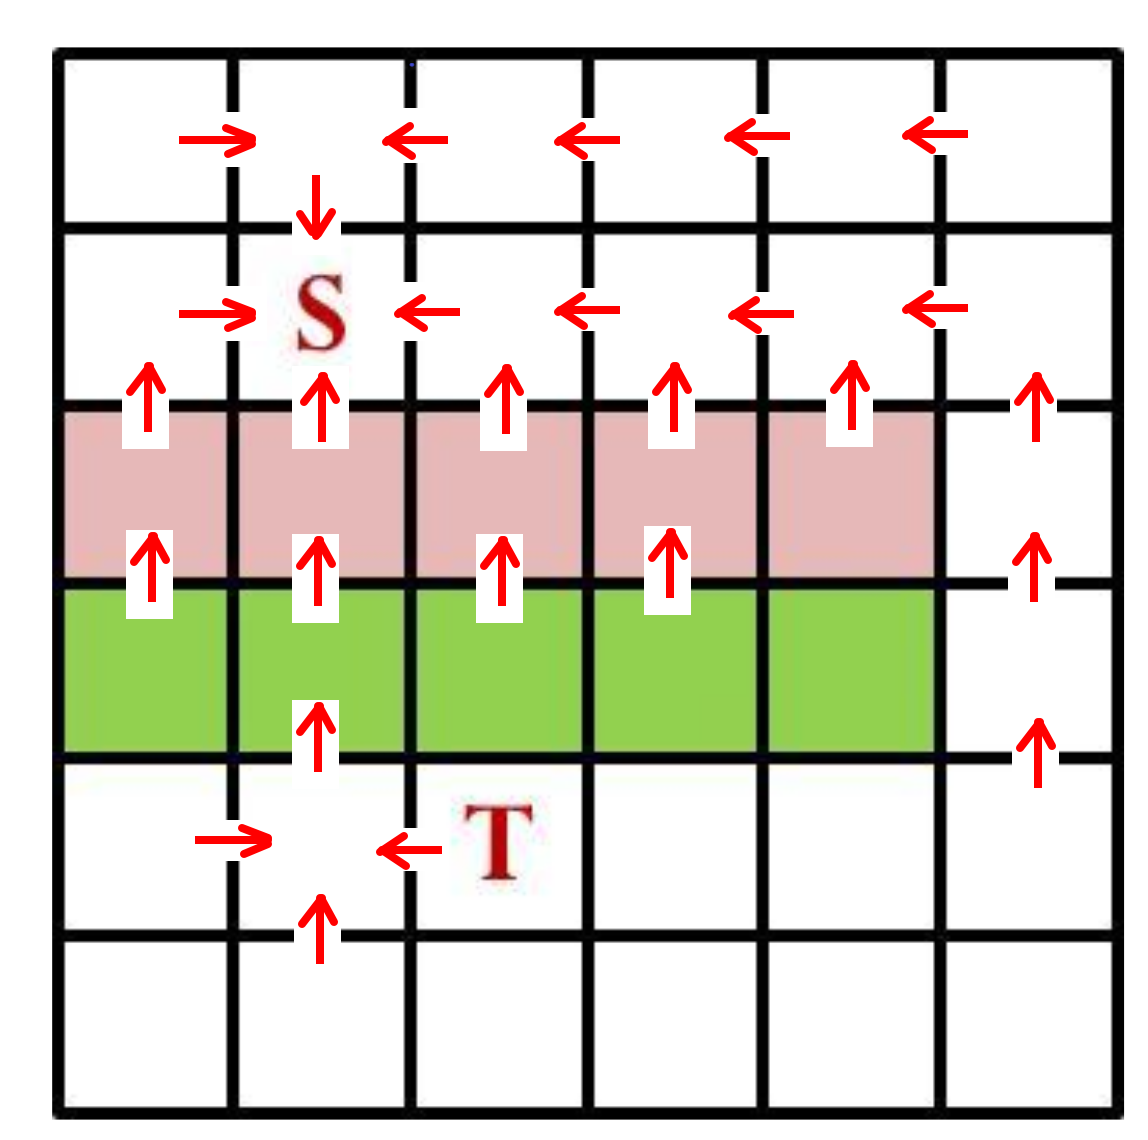
\includegraphics[width = 1.90in, height = 1.70in]{figure16.png}
        \end{center}

        The minimum pathcost is 7.


\end{document}
